\section{Formal Analysis Using Alloy}
This section provides the description of the S\&C software trough the model analysis language alloy:
\todo{revise the graph and put a screenshot of it}
\begin{lstlisting}
//SIGNATURE +++++++++++++++++++++++++++++++++++++++++++++++++++

abstract sig User{
    email: disj one Email,
    password: disj one Password
}

sig Student extends User{
	appliedTo: disj some Internship,
	student_info: disj one StudentInfo,
	feedback_of_internship: Internship -> some Feedback,
	feedback_of_platform: Feedback,
	enrolled: one University
 }

sig University extends User{
	tracked_internship : Student -> Internship,
	tracked_feedback : Internship -> Feedback,
	feedback_of_internship : Feedback -> Internship
}{this in Student.enrolled}


sig Company extends User {
    	feedback_of_internship: Feedback -> Internship,
	feedback_of_platform: Feedback
}

sig StudentInfo{
    skills: some Skills,
    cv: disj one CV
}


sig Internship{
	suitable_skills: set Skills,
	feedback_internship: disj set Feedback,
	questions: set Internship_Question,
	status: one Status_Application
}

sig Internship_Question{
	has_questions: set Question,
}{this in Internship.questions}

sig Match{
	match: Student -> some Internship
}

sig Skills{}

abstract sig Status_Application {}

sig Processed_Application extends Status_Application {}
sig Passed_Screening extends Status_Application {}
sig Rejected_Application extends Status_Application {}
sig Accepted_Application extends Status_Application {}


sig Question {
	answer: disj one Answer	
}{this in Internship_Question.has_questions}

sig Answer {
	completed: one Bool
}

sig Feedback {}

sig Email {}
sig Password {}

sig CV {
	email: disj one Email,
	skills: some Skills
}{this in StudentInfo.cv}


enum Bool {True, False}

//FACT
//++++++++++++++++++++++++++++++++++++++++++//


//Email of the student must be the same of the one inserted in the CV
fact SameEmailAsCV{
	all s: Student| one c: CV |
		c = s.student_info.cv and s.email = c.email
}

//Match between student and internship needs to have the same preferences
fact SameMatchSamePreferences{
	all m: Match | all s: Student | all i: Internship |
		s->i in m.match iff #(s.student_info.skills & i.suitable_skills) != 0
}


//The set of feedback of an internship needs to be the students' and company's ones
fact SameMatchSamePreferences{
	all m: Match | all s: Student | all i: Internship |
		s->i in m.match iff #(s.student_info.skills & i.suitable_skills) != 0
}


//Intersection between match and application must be empty
fact MatchAndApplicationDisjoint {
    all s: Student, i: Internship |
        (s -> i in Match.match) implies not (i in s.appliedTo)
}


//A student cannot apply to the same application more than one time
fact MaximumOneApplicationPerIntership{
	all s : Student | no i : Internship | i in s.appliedTo and #(i & s.appliedTo) > 1
}


//Internship question must be a subset of question
fact InternshipQuestionsSubset {
    all iq: Internship_Question | iq.has_questions in Question
}

//In order to have an Accepted_Application all answer must be completed
fact AllAnswersMustBeCompletedForAcceptedApplication {
	all i: Internship| all q: Question |
	i.status in Accepted_Application implies q in i.questions.has_questions and q.answer.completed in True
}

//The answer are available only in an Accepted_Application status
fact AnswersOnlyInAcceptedApplication {
    all i: Internship | 
        some i.questions.has_questions implies i.status in Accepted_Application
}



//Application has feedback only if its status is either Accepted_Application or Rejected_Application
fact FeedbackOnlyForAcceptedOrRejectedApplication {
    all s: Student | all i: Internship |
        some i.(s.feedback_of_internship) implies i.status in Accepted_Application or i.status in Rejected_Application
}


//Cannot add feedback to application which are not Accepted_Application
fact NoFeedbackForNonAcceptedApplication {
    all i: Internship |
        some i.feedback_internship implies i.status in Accepted_Application
}

//PREDICATES
//+++++++++++++++++++++++++++++++++++++++++++++++++++++++++++++++++++

//User add a CV
pred StudentAddCV[s: Student, cv_new: CV]
{
	s.student_info.cv = s.student_info.cv + cv_new
} 

//User remove a CV
pred StudentRemoveCV[s: Student, cv_to_remove: CV]
{
	s.student_info.cv = s.student_info.cv - cv_to_remove
}

//User updates his CV informations (email and skills)
pred NewCVInformation[s: Student,  cv_new_email: Email, skills_new: Skills]
{
    	s.student_info.cv.email = cv_new_email
	s.student_info.cv.skills = s.student_info.cv.skills + skills_new
}

//New Match has been found between a student and internship and added
pred AddNewMatch(s: Student, i: Internship, m: Match) {
    s -> i in m.match
    and s.student_info.skills & i.suitable_skills != none
}

//New feedback for an internship has been added by a student
pred NewFeedbackStudent[f_new: Feedback, s: Student, i: Internship]
{
    i.(s.feedback_of_internship) = i.(s.feedback_of_internship) + f_new
}

//New feedback has been added by a company
pred NewFeedbackCompany[f_new: Feedback, c: Company, i: Internship]
{
    (c.feedback_of_internship).i = (c.feedback_of_internship).i + f_new
}

//Every student's feeback must be tracked by his university
fact UniversityTracksFeedback {
    all s: Student, i: Internship, u: University |
        some i.(s.feedback_of_internship) implies i.(u.tracked_feedback) = i.(s.feedback_of_internship)
}

// Ensure the university tracks internships for students who have provided feedback
fact UniversityTracksInternships {
    all s: Student, i: Internship, u: University |
        some i.(s.feedback_of_internship) implies i in s.(u.tracked_internship)
}



//ASSERTION +++++++++++++++++++++++++++++++++++++++++++++++++++

assert FeedbackConsistency {
    all i: Internship | all s: Student |  all u: University |
    (i in s.appliedTo and #(i.(s.feedback_of_internship)) != 0) implies 
     i.(u.tracked_feedback) = i.(s.feedback_of_internship) and i in s.(u.tracked_internship)
}

assert ValidMatch {
    all m: Match | all s: Student | all i: Internship |
    s -> i in m.match implies s.student_info.skills & i.suitable_skills != none
}


pred simpleWorld{
	#Student = 1
	#University = 1
	#Company = 1
	#Internship = 1
	#Internship_Question = 1
	#Question = 1
	#StudentInfo = 1
	#Skills = 1
}

//TO RUN ASSERTION AND PREDICATES

run StudentAddCV for 4

run StudentRemoveCV for 4

run NewCVInformation for 4

run AddNewMatch for 4

run NewFeedbackStudent for 4

run NewFeedbackCompany for 4

check FeedbackConsistency

check ValidMatch

run simpleWorld for 5

\end{lstlisting}



\begin{figure}
    \centering
    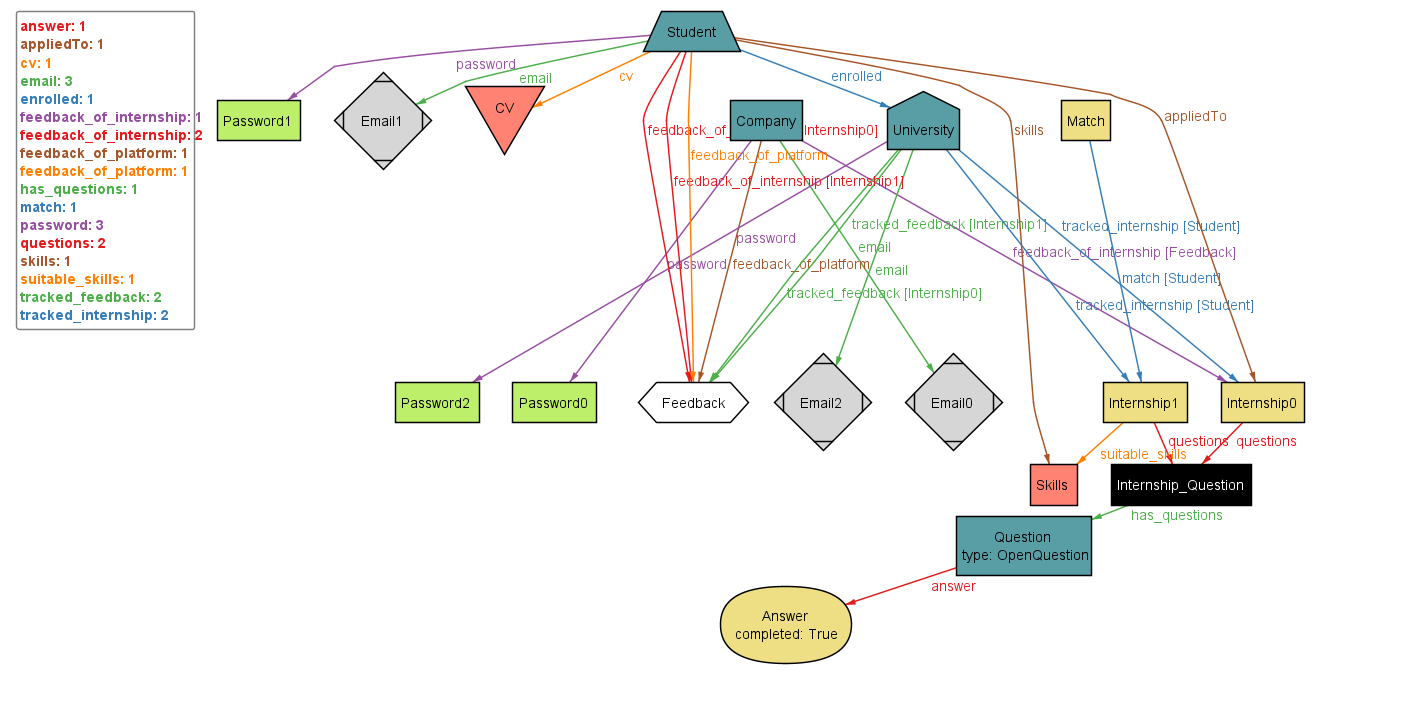
\includegraphics[angle=270, width=0.65\linewidth]{images/AlloySimpleWorld.png}
    \caption{Simple world description in Alloy}
    \label{fig:simple-world}
\end{figure}



\pagebreak
